\section{Dissipation from trajectories alone}
\label{sec:estimators}

Everything above used the generator. Data never provides it: only an observed
sequence of profiles. Two estimators bridge the gap, each validated against
the exact Schnakenberg meter on synthetic Glauber trajectories \emph{before}
any data contact (unit \texttt{thermo.estimators}; red-team signed off after
one blocking objection, disclosed below).

\paragraph{Sampling identity.} We simulate by uniformisation: the skeleton
chain $P = I + L/\Lambda$ stepped with $\mathrm{Exp}(\Lambda)$ holding times.
Two exact facts make the skeleton the right estimation object: it shares the
chain's stationary law, and its per-step entropy production equals
$\EPR/\Lambda$; moreover the $(k{+}1)$-block KLD of a stationary Markov chain
equals $k$ times the per-step entropy production, so the estimator below has a
sharp target at every $k$.

\paragraph{KLD $k$-th order Markov \citep{roldan2010}.} The plug-in
$\hat\sigma^{(k)} = \frac{1}{k\tau}\sum P(Y_{0:k}) \log
P(Y_{0:k})/P(Y_{k:0})$ recovers the exact meter with Spearman $\rho = 1.0$
and $\sim 1\%$ per-level error across the ten-$\alpha$ family
(Figure~\ref{fig:est}, left), and reads $< 5\times10^{-3}$ on exact potential
games (pure plug-in bias; truth is $0$). It is data-hungry: the identity is a
population statement, and with $n \not\gg n_{\rm states}^{k+1}$ the estimator
\emph{underestimates} ($k=4$ reads $\sim 17\%$ low at our validation sample
size; the failure mode is itself a regression test).

\paragraph{TUR lower bound \citep{barato2015,horowitz2017}.} From the first
two cumulants of a time-integrated current $J_T$:
$\EPR \ge 2\langle J_T\rangle^2 / (\mathrm{Var}(J_T)\, T)$. A certified bound
rather than a point estimate --- a poor current choice loosens but never breaks
it --- which makes it the designated headline number for partially observed
data \citep{otsubo2022}. Three methodological facts were learned adversarially
and are now tests:
(i) the bound is a \emph{fixed-horizon} statement --- fixing the jump count
instead suppresses the Poisson timing fluctuation and inflated the ``bound''
$1.5\times$ above the true EPR before we caught it;
(ii) at $M$ windows the sample version carries $+\mathrm{Var}/M$ and
Jensen-on-$1/\widehat{\mathrm{Var}}$ biases, both now corrected;
(iii) even debiased, the \emph{point} estimate legitimately straddles the
truth near equilibrium, where the TUR saturates --- it exceeded the exact EPR
at 2 of 10 sweep levels (max ratio $1.073$). The certified statement is the
lower bootstrap quantile, which stayed below the exact EPR at every level.
The initial artifact language called the point estimate a certified bound;
the red-team blocked the gate until the distinction was made structural
(a separate \texttt{tur\_epr\_bound\_ci} API) --- we record this because the
correction is part of the result.

\begin{figure}[t]
\centering
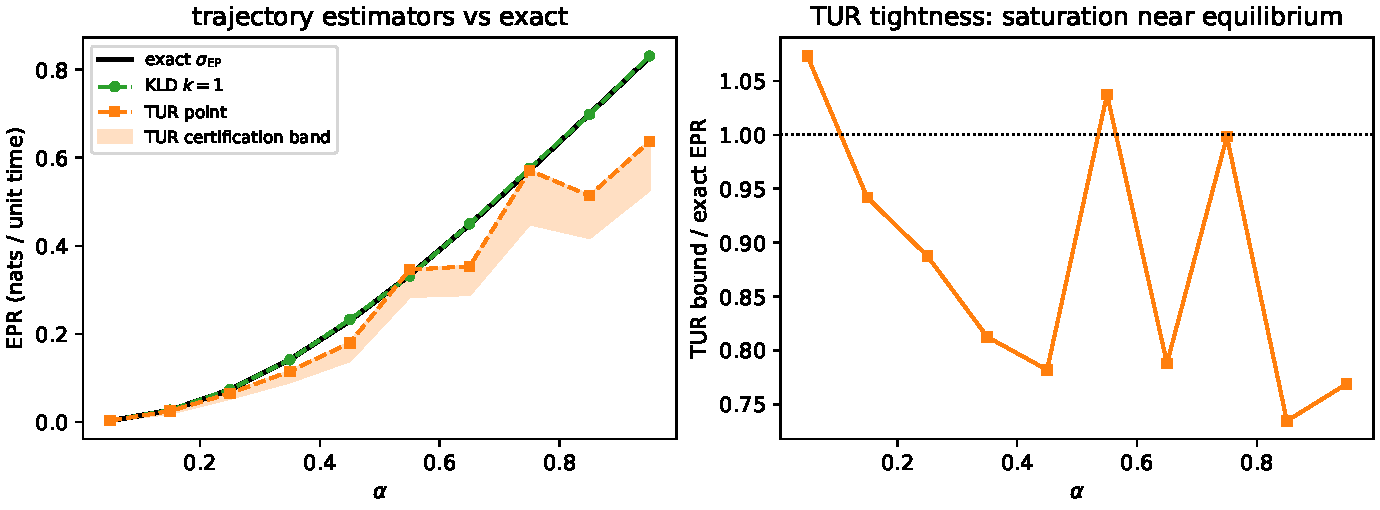
\includegraphics[width=\linewidth]{figures/estimator_tracking.pdf}
\caption{Left: exact EPR vs.\ its trajectory estimators along $\alpha$
($\lambda=1.5$; KLD from $8\times 60$k stationary steps, TUR from 128
fixed-horizon windows). Right: TUR tightness --- the bound saturates near
equilibrium and degrades gracefully (and conservatively) as the drive grows.
Artifact: \texttt{estimator\_alpha\_sweep.json}.}
\label{fig:est}
\end{figure}

\paragraph{Tightness is a diagnostic.} The bound/exact ratio is $\approx
0.97$ at $\alpha = 0.05$ (linear-response saturation) and drifts to
$0.6$--$0.7$ by $\alpha = 0.95$ (Figure~\ref{fig:est}, right): the TUR is
tightest exactly where dissipation is smallest, i.e.\ it loses efficiency
precisely where there is more to measure --- the right failure direction for a
conservative instrument.
